\documentclass{beamer}

% does not look nice, try deleting the line with the fontenc.
\usepackage[english]{babel}
\usepackage{amsmath}
\usepackage[latin1]{inputenc}
\usepackage{units}
\usepackage{colortbl}
\usepackage{multimedia}
\usepackage{bm}
\usepackage{subcaption}
\usepackage{algorithm2e}
\usepackage{algorithmic}

\mode<presentation>
{
  \usetheme{Boadilla}
  \useoutertheme{infolines}
  \setbeamercovered{transparent} 
}
	

\title[Dynamical systems \& deep learning]{\textsc{Dynamical systems modeling with deep learning tools}}


\author[]{Marco Forgione, Dario Piga}

\institute[IDSIA]{IDSIA Dalle Molle Institute for Artificial Intelligence USI-SUPSI, Lugano, Switzerland} 


\date[]{April 15, 2021}


\subject{System Identification, Deep Learning, Machine Learning, Regularization}


%% MATH DEFINITIONS %%
\newcommand{\So}{S_o} % true system
\newcommand{\hidden}[1]{\overline{#1}}
\newcommand{\nsamp}{N}
\newcommand{\Yid}{Y}
\newcommand{\Uid}{U}
\newcommand{\Did}{{\mathcal{D}}}
\newcommand{\tens}[1]{\bm{#1}}

\newcommand{\batchsize}{q}
\newcommand{\seqlen}{m}
\newcommand{\nin}{n_u} 
\newcommand{\ny}{n_y} 
\newcommand{\nx}{n_x}

\newcommand{\NN}{\mathcal{N}} % a feedforward neural network

\newcommand{\norm}[1]{\left \lVert #1 \right \rVert}
\DeclareMathOperator*\argmin{arg \, min}
\newcommand{\Name}{\emph{dynoNet}}


%% DYNONET MATH DEFINITIONS %%
\newcommand{\q}{q} % shift operator
\newcommand{\A}{A} % autoregressive polynomial
\newcommand{\ac}{a} % autoregressive polynomial coefficient
\newcommand{\B}{B} % exogenous polynomial
\newcommand{\bb}{b} % exogenous polynomial coefficient
\newcommand{\Gmat}{\mathbb{G}} % transfer function operator in matrix form
\newcommand{\tvec}[1]{\bm{#1}}
\newcommand{\mat}[1]{\bm{#1}}
\newcommand{\sens}[1]{\tilde{#1}}
\newcommand{\adjoint}[1]{\overline{#1}}
\newcommand{\loss}{\mathcal{L}}
\newcommand{\pdiff}[2]{\frac{\partial #1}{\partial #2}}
%\newcommand{\nsamp}{T}

\newcommand{\conv}{*}
\newcommand{\ccorr}{\star}
\definecolor{orange}{RGB}{204, 85, 0}
%% DYNONET %%

\definecolor{darkgreen}{RGB}{20,150,50}
\definecolor{Periwinkle}{rgb}{0.0, 0.0, 0.0}
\usepackage{listings}
\newcommand{\book}{\includegraphics[width=10pt]{img/proceeding-logo.jpg}}
\newcommand{\github}{\includegraphics[width=10pt]{img/github-logo.jpg}}
\begin{document}

\begin{frame}
  \titlepage
\end{frame}

%%% DYNONET %%%

\begin{frame}{Context}
 The connection between \structure{deep learning} and \structure{dynamical system} theory is under intensive investigation:%. Examples:
 %Several contributions deal with:
 \vskip 1em
 \begin{itemize}
  \item Analysis of deep architectures through the lens of system theory
   \begin{itemize}
	\item[\book]
		\begin{tiny}
	\structure{E. Haber and L. Ruthotto},
      Stable architectures for deep neural networks. \vskip -1em
     \emph{ Inverse Problems, 2017}
		\end{tiny}\\	
    \end{itemize}
  \item Dynamical systems as deep learning layers
 	\begin{itemize}
	\item[\book]
		\begin{tiny}
	\structure{T. Q. Chen, Y. Rubanova, J. Bettencourt, D. K. Duvenaud,}
     Neural Ordinary Differential Equations. \vskip -1em
     In: \emph{Advances in Neural Information Processing Systems, 2018}
		\end{tiny}\\	
    \end{itemize}
  \item Modeling of dynamical systems with deep learning tools % and algorithms
 	\begin{itemize}
	\item[\book]
		\begin{tiny}
	\structure{M. Raissi, P. Perdikaris, G. E. Karniadakis,}
     Physics-informed neural networks: A deep learning framework for solving forward and inverse problems
involving nonlinear partial differential equations. \vskip -1em
     \emph{Journal of Computational Physics, 2019}
		\end{tiny}\\	
    \end{itemize}
  \end{itemize}
\vskip 1em
This connection is beneficial to both fields.
\end{frame}

\begin{frame}{Residual Networks \& Dynamical Systems}
 A \structure{Residual Network} is equivalent to the forward Euler integration of an underlying continuous-time \structure{neural dynamics} 
 \begin{columns}
 \column{.5\textwidth}
% \pause
%\only<1>{
%\begin{figure}
%\centering
%\vskip 2em
%\includegraphics[height=35pt]{img/blank.pdf}
%\includegraphics[height=35pt]{img/misc/forward_euler.pdf}
%\end{figure}
%}
%\only<1->{
\begin{figure}
\centering
\includegraphics[height=35pt]{img/misc/forward_euler.pdf}
\end{figure}
%}
 \column{.5\textwidth}
\begin{align*}
 x_{k+1} &= x_k + \mathcal{N}_f(x_k)\Delta t
\end{align*}
\end{columns}
\vskip 2em
\pause
Corresponding ordinary differential equation (ODE):
\begin{equation*}
\dot x = \mathcal{N}_f(x)
\end{equation*}
\pause
Related questions:
\begin{itemize}
\item Stability/well-posedness of the ResNet related to the ODE?
\item Is the neural ODE a useful layer for deep learning?
\item Are deep learning tools  useful for dynamical systems modeling?%How to model dynamical systems using neural networks?
\end{itemize}
\end{frame}


\begin{frame}{}{}
\begin{center}
\huge{\structure{Tailor-made state-space neural model structures}}
%\vskip 1em
%\begin{small}
%\texttt{marco.forgione@idsia.ch}
%\end{small}
\end{center}
\end{frame}

\begin{frame}{Motivations}

\structure{Neural state-space models} (Recurrent Neural Networks) are widely used for dynamical systems. 
However, they seldom exploit \structure{a priori knowledge}. %\\
%\vskip 1em
%Training RNNs requires a \structure{sequential simulation} through the training time steps, which can be slow. 
%How to parallelize the training procedure?
\vskip 2em
\pause
We present:
\begin{itemize}
\item {tailor-made} neural model structures for system identification;
\item {efficient algorithms} to fit these model structures to data. 
\end{itemize}

\vskip 1.0 em
\pause
 	\begin{itemize}
	\item[\book]
		\begin{tiny}
	\structure{M.~Forgione and D.~Piga.}
    Continuous-time system identification with neural networks: model structures and fitting \vskip -1em
    criteria. \emph{European Journal of Control, 59(2021), pp 69-81}
		\end{tiny}\\								

 	\item[\book]
		\begin{tiny}
	\structure{B.~Mavkov, M.~Forgione and D.~Piga.}
									Integrated Neural Networks for Nonlinear Continuous-Time System Identification.
									\vskip -1em
									\textcolor{Periwinkle}{\textit{IEEE Control Systems Letters, 4(4), pp 851-856, 2020.}}
		\end{tiny}\\								
	\item[\book]
		\begin{tiny}
	\structure{M. Forgione and D.~Piga.}
				Model structures and fitting criteria for system identification with neural networks.
				\vskip -1em
				\textcolor{Periwinkle}{\textit{In Proc. of the 14th. IEEE Application of Information and Communication Technologies Conference (AICT), 2020}}
		\end{tiny}\\	
    \pause
    \item[\github]\begin{tiny}{\url{https://github.com/forgi86/sysid-neural-continuous}}\end{tiny}
     \item[\github]\begin{tiny}{\url{https://github.com/bmavkov/INN-for-Identification}}\end{tiny}
    \item[\github]\begin{tiny}{\url{https://github.com/forgi86/sysid-neural-structures-fitting}}\end{tiny}
	\end{itemize}
	
\end{frame}

\begin{frame}{Settings}
The \structure{true system} is assumed to have a state-space representation:
\begin{equation*}
\begin{split}
 \dot x(t) &= f(x(t), u(t)) \\
 y^{\text o}(t)  &= g(x(t)),\\
\end{split}
\end{equation*}
with noisy discrete-time measurements available: $y_k = y^{\text o}(t_k) + e_k$.
\pause
\vskip 1em
\structure{Training dataset} $\Did$: a single input/output sequence with:
\begin{itemize}
\item input samples $\Uid = \{u_{0},\;u_{1},\dots,\;u_{\nsamp-1}\}$
\item output samples  $\Yid = \{y_{0},\;y_{1},\dots,\;y_{\nsamp-1}\}$ 
\item time instants $T = \{t_{0},\;t_{1},\dots,\;t_{\nsamp-1}\}$ 
\end{itemize}
\vskip 1em
\pause
\structure{Objective}: estimate a dynamical model of the system.
\end{frame}


\begin{frame}{Neural Dynamical Models}{}
A very \structure{generic} neural model structure:
%\begin{align*}
% x_{k+1} &= \NN_f(x, u;\;\theta)\\
%    y_k  &= \NN_u(x; \theta)
%\end{align*}
\begin{align*}
 \dot{x} &= \NN_f(x, u;\;\theta)\\
    y  &= \NN_g(x; \theta)
\end{align*}

where $\NN_f$, $\NN_g$ are feed-forward neural networks.\\
\vskip 1em\
\pause
Can be  \structure{specialized}, according to available system knowledge:
\begin{itemize}
  \item State fully observed $\Rightarrow$ 
  \begin{align*}
 \dot x &= \NN_f(x, u;\;\theta)\\
    y  &= x
\end{align*}
%   \pause
%  \item Linear approximation available $\Rightarrow$
% \begin{equation*}
% \begin{split}
%  \dot x &= A x + B u + \NN_f(x_{k}, u_{k}; \theta)\\
%  y     &= C x + \NN_g(x, u; \theta)
%  \end{split}
% \end{equation*}
\item ...
 \end{itemize}
\end{frame}

\begin{frame}{Neural Dynamical Models}{Physics-inspired model structures}
%\vskip 1em
 Two-tank system. Input: flow $u$ in upper tank, output: lower tank level $x_2$.
 \begin{columns}
  \column{.6\textwidth}
  \begin{itemize}
   \item The system has two states: $x_1$ and $x_2$
   \item State $x_1$ does not depend on $x_2$
   \item State $x_2$ does not depend directly on $u$
   \item The state $x_2$ is measured
   \end{itemize}
  \column{.3\textwidth}
  \begin{center}
  \includegraphics[width=.6\textwidth]{img/CTS/CTS_scheme.pdf}
  \end{center}
\end{columns}
 %\pause
 \vskip 2em
 These observations are embedded in the \structure{physics-inspired} neural model:
% \begin{columns}
% \column{.5\textwidth}
\vskip -1.5em
\begin{small}
 \begin{align*}
  \dot x_1 &= \mathcal{N}_{1}(x_1, u;\;\theta)\\
  \dot x_2 &= \mathcal{N}_{2}(x_1, x_2;\;\theta)\\
  y        &= x_2
 \end{align*}
\end{small}
%  \column{.5\textwidth}
\vskip -2em
%\end{columns}
\end{frame}


\begin{frame}{Training Neural Dynamical Models}
How to fit the network efficiently to a single, \structure{long training sequence}?\\
How to split it in sub-sequences for \structure{minibatch training}?\\%, taking into account the initial conditions?
%For each iteration of \structure{gradient-based} optimization:
\begin{figure}
\centering
\includegraphics[width=.8\textwidth]{img/scheme/scheme_multistep_plain.pdf}
\end{figure}
\pause
Problem: how do we choose $\hat {\tens{x}}_{:, 0}$, the \structure{initial state} for each sub-sequence? \\
We need it to initialize all simulations.
\end{frame}

\begin{frame}{Training Neural Dynamical Models}
We consider the unknown state sequence $\hidden{X}$ as an \structure{optimization variable}.\\
We sample from $\hidden{X}$ to obtain the initial state for simulation in each batch. 
 \begin{figure}
\centering
\includegraphics[width=.8\textwidth]{img/scheme/scheme_multistep_state_est.pdf}
\end{figure}
%\pause
$J^{\rm fit}$ is now a function of both $\theta$ and $\hidden{X}$. We optimize w.r.t. both!
\end{frame}

\begin{frame}{Training Neural Dynamical Models}
The hidden state sequence $\hidden{X}$ should also satisfy the identified dynamics!
We enforce this by adding a \structure{regularization term} in the cost function.
 \begin{figure}
\centering
\includegraphics[width=.8\textwidth]{img/scheme/scheme_multistep_with_reg.pdf}
\end{figure}
%\pause
We minimize a \structure{weighted sum} of $J^{\rm fit}$ and $J^{\rm reg}$ w.r.t. both $\theta$ and $\hidden{X}$.
\end{frame}

% \begin{frame}{Training Neural Dynamical Models}{}
%  For each iteration of gradient-based optimization:
%  \begin{enumerate}
% \item \textbf{extract} batch start index vector $s \in \mathbb{N}^\batchsize, s_j < \nsamp - m$
% \item \textbf{define} from $\Did = \{Y,U,T,\hidden{X}\}$:
% \begin{itemize}
% \item output tensor $\tens {y} \in \mathbb{R}^{\batchsize \times \seqlen \times \ny}\qquad\qquad$ where $\tens{y}_{j,h} = Y_{s_{j}+h}$ 
% \item input tensor $\tens {u} \in \mathbb{R}^{\batchsize \times \seqlen \times \nin}\qquad\;\;\;\;\;\;\;\;\;$ 
% where $\tens{u}_{j,h} = U_{s_{j}+h}$
% \item relative time tensor $\tens {\tau} \in \mathbb{R}^{\batchsize \times \seqlen \times \nin}\;\;\;\;\;$ where 
% $\hidden{\tens{\tau}}_{j,h} = {T}_{s_{j}+h}$ 
% \item hidden state tensor $\hidden{\tens {x}} \in \mathbb{R}^{\batchsize \times \seqlen \times \nx}\;\;\;\;\;\;$ where 
% $\hidden{\tens{x}}_{j,h} = \hidden{X}_{s_{j}+h}$ 
% \item initial condition $\hat{\tens{x}}_{:,0}\qquad \qquad \qquad\;\;\;\;\;$ where 
% $\hat{\tens{x}}_{j,0}= \hidden{x}_{s_j}$
% \end{itemize}
% \pause
% \item \textbf{simulate} $\hat {\tens{y}}_{j,h}$
% \begin{align*} 
%      \hat {\tens{x}}_{j}(\tau) &= {\rm ODEINT}(\tau, \mathcal{N}_f(\cdot, \cdot; \theta), \tens{x}_{j,0})\\
%  	 \hat {\tens{y}}_{j,h}  &= \NN_g(\hat {\tens x}_{j}(\tvec{\tau}_{jh}))
% %    \hat {\tens{x}}_{j, t+1} &= \hat {\tens x}_{j, t} + \NN_f(\hat {\tens x}_{j, t}, u_j, t)\\
% %	\hat {\tens{y}}_{j,t}  &= \NN_g(\hat {\tens x}_{j, t})
% \end{align*} 
% \vskip -.5em
% \pause
% \vskip -.5em
%   \item \textbf{compute} the loss
% $J(\theta, \hidden{X}) = \overbrace{\norm{\hat{\tens{y}} - {{\tens{y}}}}^2}^{J^{\rm fit}} + \alpha \overbrace{\norm{\hat{\tens{x}} - {{\hidden{\tens{x}}}} }^2}^{J^{\rm reg}}
% $
% \pause
% \item \textbf{perform} gradient-based step (back-propagation) to minimize the cost
% \end{enumerate}
% \end{frame}


\begin{frame}{Example}{RLC circuit}
 We consider a nonliner \structure{RLC circuit}:
 \begin{columns}
 \column{.5\textwidth}
\footnotesize
 \begin{equation*}
\begin{bmatrix}
\dot v_C\\
\dot i_L
\end{bmatrix} = 
\begin{bmatrix}
  0           & \tfrac{1}{C}\\
 \tfrac{-1}{L(i_L)} & \tfrac{-R}{L(i_L)}\\
\end{bmatrix}
\begin{bmatrix}
v_C\\
i_L
\end{bmatrix} +
\begin{bmatrix}
0\\
\tfrac{1}{L(i_L)}
\end{bmatrix} 
v_{in}
\end{equation*}
 \column{.5\textwidth}
 \vskip -2em
\begin{figure}
\centering
\includegraphics[width=.7\linewidth]{img/RLC/RLC.pdf}
\end{figure}
\end{columns}
\vskip 1em
with %$R = 3~\Omega$, $C=270~\text{nF}$, and 
\structure{nonlinear inductance} $L(i_L)$
\vskip -1em
\begin{columns}
 \column{.5\textwidth}
\footnotesize
 \begin{equation*}
 L(i_L) = L_0\bigg[\bigg(\frac{0.9}{\pi}\!\arctan\!\big(-\!5(|i_L|\!-\!5\big)+0.5\bigg) + 0.1 \bigg]%~\text{H}
\end{equation*}
 \column{.5\textwidth}
\begin{figure}
\centering
\includegraphics[width=.5\linewidth]{img/RLC/RLC_characteristics.pdf}
\end{figure}
 \end{columns}
%\pause
\vskip 0.5em
Input: voltage $v_{in}$.  Output: voltage $v_C$, current $i_L$. \text{SNR}=20 \\%Datasets:
%\begin{itemize}
%\item identification: $N\!=\!4000$, filtered w.n. $\sigma_v\!=\!80~V$, $B_v\!=\!150~kHz$
%\item validation: $N\!=\!4000$,  $v_{in}$ filtered w.n. $\sigma_v\!=\!60~V$, $B_v\!=\!%200~kHz$
%\end{itemize}
\pause
\vskip .5em
Neural model structure: \structure{fully observed state}
\begin{equation*}
\begin{split}
 \dot x &= \NN_f(x, u; \theta)\\
 y    &= x
 \end{split}
\end{equation*}
\end{frame}




\begin{frame}{Example}{RLC circuit}
Results  on the test dataset. Training with:
\vskip 1em
\begin{columns}
  \column{.5\textwidth}
  \centering
  $q=64$ sequences of length $m=64$ %, %$\text{SNR}=20~\text{dB}$
  \includegraphics[width=\textwidth]{img/RLC/RLC_SS_val_64step_noise.pdf}
  train time: 320~s
  \column{.5\textwidth}
    \centering
    $q=1$ sequence of length $m=4000$
  %simulation error minimization\\ %$\text{SNR}=20~\text{dB}$
  \includegraphics[width=\textwidth]{img/RLC/RLC_SS_val_64step_noise.pdf}
  \alert{train time: 7000~s}
  \end{columns}
\end{frame}

\begin{frame}{Example}{Cascaded Tank System}
Dataset with \structure{real measurements} from \url{www.nonlinearbenchmark.org}
%\vskip 1em
\begin{columns}
 \column{.5\textwidth}
% System equations (no overflow)
% \begin{equation*}
%  \begin{split}
%   \dot x_1 &= -k_1\sqrt{x_1} + k_4 u\\
%   \dot x_2 &= k_2 \sqrt{x_1} - k_3 \sqrt{x_2}\\
%   y  &= x_2
%  \end{split}
% \end{equation*}
\begin{figure}
\centering
\includegraphics[height=.5\linewidth]{img/CTS/CTS.jpg}
\end{figure}
 \column{.5\textwidth}
\begin{figure}
\centering
\includegraphics[height=.5\linewidth]{img/CTS/CTS_scheme.pdf}
\end{figure}
\end{columns}
\vskip .5em
%\pause
 Neural model structure: \structure{physics-inspired}
 \vskip -1.45em
\begin{align*}
 \dot x_1 &= \NN_{1}(x_1, u; \theta)\\
 \dot x_2 &= \NN_{2}(x_1, x_2, \alert{u}; \theta)\\
 y        &= x_2
\end{align*}
%\vskip -.5em
\pause
The dependency of $\NN_2$ on $u$ models \alert{water overflow} from upper tank.
%We could embed more insight (e.g., state $x_1$ does not depend on $x_2$\dots)
%Identification and validation datasets with $N=1024$ samples
\end{frame}

\begin{frame}{Numerical example}{Cascaded Tank System}
Training with $q=64$ subsequences of length $m=128$. Results on:% the ident/test datasets.\\
%Train time: 183~s
\vskip 1em
\begin{columns}
  \column{.5\textwidth}
  \centering
  Training dataset
  \includegraphics[width=\textwidth]{img/CTS/CTS_SS_id_model_SS_256step.pdf}
  $R^2 = 0.99$,\;$\text{RMSE}=0.08~\text{V}$
  \column{.5\textwidth}
    \centering
  Test dataset
  \includegraphics[width=\textwidth]{img/CTS/CTS_SS_val_model_SS_256step.pdf}
  $R^2 = 0.97$,\;$\text{RMSE}=0.33~\text{V}$
  \end{columns}
\end{frame}

\begin{frame}{Conclusions}{}
We have presented \structure{tailor-made} neural structures for system identification embedding a priori knowledge.
\vskip 1em
We have shown how to parallelize the training using batches of short-size \structure{subsequences}, and taking into account the effect of the \structure{initial condition}.
\pause
\vskip 2em
Current/Future work
\begin{itemize}
 \item Estimation and control algorithms
 \item Learning of Partial Differential Equations
\end{itemize}

\end{frame}

\end{document}
